
\section{LTE}
Long Term Evolution (4G),perfomance:
\begin{itemize}
	\item Up to 300 Mbit/s downlink, 75Mbit/s uplink
	\item 5-20ms latency
\end{itemize}
\subsection{Origin}
It is expected that performance in UMTS has reached it limits:
\begin{itemize}
	\item Higher transfer rates would have required higher chip
	rate $\to$ shorter chip duration $\to$ more sensitive to
	multipath fading
	\item Latency in UMTS still highn partially because of old
	design (GPRS based network)
\end{itemize}
LTE is a complete redesign, its a simplified IP-only network with
gateways to other networks.

\subsection{Radio Interface}
LTE use a completely new radio interface called OFDM and SC-FDMA
\subsubsection{Downlink}
OFDM (Orthogonal frequency-division multiplexing):
\begin{itemize}
	\item Data is distributed over a large number (up to 1200) of 15 kHz
	space orthogonal subcarriers
	
\end{itemize}
Subcarriers are orthogonal if the maximum amplitude of one subcarrier
is reached while the other subcarriers amplitude is zero	
\begin{description}
	\item[Advantages:] More robust against interferences that affect only a 
	few subcarriers.
	
	\item[Disadvantage:] More coding work, power consumption increases
	with number of subcarriers (does'nt matter for base station)

\end{description}

\subsubsection{Uplink}
SC-FDMA( Single Carrier FDMA)
\begin{itemize}
	\item Comparable to OFDM, but data is preprocessed in a wat that 
	Peak-To-Average-Power Ration of the signal is smaller than with 
	OFDM

\end{itemize}
$\to$ More energy-efficient (but lower uplink rate)

\subsection{Category and Bearer}
User equipment are category and depending on their category 
different aspect in transmission will change: modulation, peak data rate,MIMO,\ldots\\
UE request different bearer to specify its traffic requirements of application (QoS)

\subsection{Network}
\begin{figure}[ht!]
	\centering
	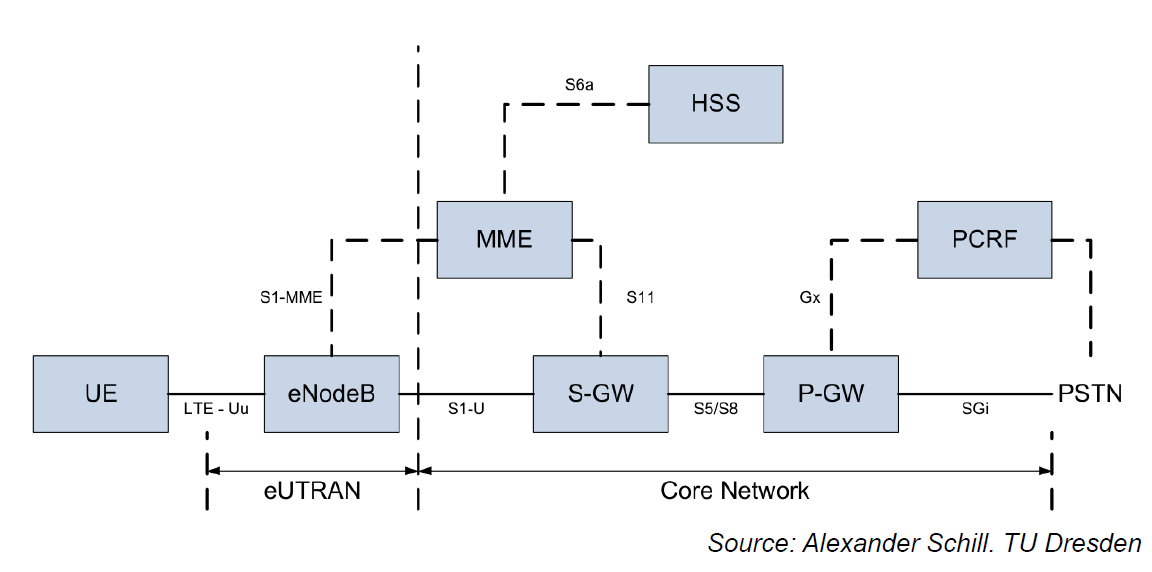
\includegraphics[scale=0.5]{img/lte.png}
	\caption{UE=User Equip.=MS, HSS = Home Subscriber Server=HLR}
\end{figure}

\subsubsection{eNodeB}
eNodeB = evolved Node B, does the job of BTS,BSC,Node B and RNC. eNodeB can 
directly communicate with each other:
\begin{description}
	\item[Interference coordination] UE reports signal measurements from neighbor 
	cells to its eNodeB; the node can contact the eNodeB of those cells
	\item[Handover] eNodeB can decide and prepare handover 
	(without involvement of an MSC in GSM)
\end{description}

\subsubsection{P-GW}
An UE gets an IP address assigned by the P-GW in the moment it connects 
to the LTE network.
\begin{description}
	\item[P-GW(Packet Data Network Gateway:] Connects to the Internet
	or Intranets of large companies
\end{description}

\subsubsection{S-GW}
Incoming Internet traffic is tunneled from the P-GW to the S-GW and then to 
the eNodeB of the UE.
\begin{itemize}
	\item[S-GW(Servicing Gateway):] Responsible for several eNodeB
\end{itemize}

\subsubsection{MME}
\begin{description}
	\item[MME (Mobility Management Entity]
	\begin{itemize}
		\item Authentication
		\item Establishing tunnels and modifyinh them if handover
		\item Helping to handover if two eNodeB cannot communicate to each other
	\end{itemize}

\end{description}
\subsection{LTE Advanced}
\begin{itemize}
	\item Up to 1Gbit/s downlink
	\item Pico and Femto cells for crowded areas
	\item Carrier bundling
	\item 4x8 MIMO

\end{itemize}
